\documentclass{article}
\usepackage{booktabs}
\usepackage{graphicx}
\usepackage{amsmath, amsfonts}
\usepackage{pdflscape}
\usepackage{tikz}

\begin{document}

\begin{landscape}

% Requires the booktabs if the memoir class is not being used
\begin{table}[htbp]
   \centering
   \caption{Overview of different entropy measures of simple models with different structures. The columns from left to right represent a schematic representation of the model structure, its mathematical representation, entropy rate per jump $\theta_J$, mean number of jumps $\mathbb{E} [\mathcal{N}]$, entropy rate per unit time $\theta$, mean transit time $\mathbb{E} [\mathcal{T}]$, and path entropy $\mathbb{H} (\mathcal{P})$. Underlined numbers are the highest values per column }
   \begin{tabular}{@{} ccccccr @{}} % Column formatting, @{} suppresses leading/trailing space
      \toprule
      Structure    & $\frac{\mathrm{d}}{\mathrm{d}t} \mathbf{x} (t)$ & $\theta_J$ & $\mathbb{E} [\mathcal{N}]$ & $\theta$ & $\mathbb{E} [\mathcal{T}]$ & $\mathbb{H} (\mathcal{P})$ \\
      \midrule
       %\documentclass{standalone}
%\usepackage{tikz}
%
%\begin{document}

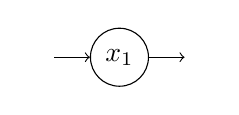
\begin{tikzpicture}
\node at (-1, 0) [shape=circle] (in) {};
\node at (0, 0) [shape=circle, draw] (x1) {$x_1$};
\node at (1, 0) [shape=circle] (out) {};
\draw [->] (in) to  (x1);
\draw [->] (x1) to (out);
\end{tikzpicture}

%\end{document}
  & $-\lambda x +1$ & $0.5 \ (1 - \log \lambda)$ & 2.00 & $\lambda (1 - \log \lambda)$ & $1/ \lambda$ & $1 - \log$ \\
       \input{Compartments/twoseries.tex}    & $\left( \begin{matrix} -1 & 0 \\ 1 & -1  \end{matrix} \right) x + \left( \begin{matrix} 1 \\ 0 \end{matrix} \right)$ & 0.67 & 3.00 & 1.00 & 2.00 & 2.00  \\
         \input{Compartments/twoparallel.tex}  & $\left( \begin{matrix} -1 & 0 \\ 0 & -1  \end{matrix} \right) x + \left( \begin{matrix} 1 \\ 1 \end{matrix} \right)$ & 0.85 & 2.00 & 1.69 & 1.00 & 1.69 \\
         \input{Compartments/twofeedback1.tex}  & $\left( \begin{matrix} -1 & 1/2 \\ 1 & -1  \end{matrix} \right) x + \left( \begin{matrix} 1 \\ 0 \end{matrix} \right)$ & 1.08 & 5.00 & 1.35 & \underline{4.00} & \underline{5.39} \\
         %\documentclass{standalone}
%\usepackage{tikz}
%
%\begin{document}

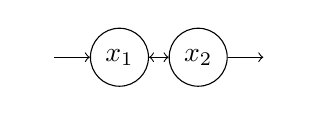
\begin{tikzpicture}
\node at (-1, 0) [shape=circle] (in) {};
\node at (-1, -0.5) [shape=circle] (out1) {};
\node at (0, 0) [shape=circle, draw] (x1) {$x_1$};
\node at (1, 0) [shape=circle, draw] (x2) {$x_2$};
\node at (2, 0) [shape=circle] (out2) {};
\draw [->] (in) to  (x1);
% \draw [->] (x1) to (out1);
\draw [<->] (x1) to (x2);
\draw [->] (x2) to (out2);
\end{tikzpicture}

%\end{document}

   & $\left( \begin{matrix} -1 & 1/2 \\ 1/2 & -1  \end{matrix} \right) x + \left( \begin{matrix} 1 \\ 1 \end{matrix} \right)$ & \underline{1.36} & 3.00 & 2.04 & 2.00 & 4.08 \\
         %\documentclass{standalone}
%\usepackage{tikz}
%
%\begin{document}

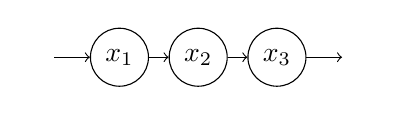
\begin{tikzpicture}
\node at (-1, 0) [shape=circle] (in) {};
\node at (0, 0) [shape=circle, draw] (x1) {$x_1$};
\node at (1, 0) [shape=circle, draw] (x2) {$x_2$};
\node at (2, 0) [shape=circle, draw] (x3) {$x_3$};
\node at (3, 0) [shape=circle] (out) {};
\draw [->] (in) to  (x1);
\draw [->] (x1) to (x2);
\draw [->] (x2) to (x3);
\draw [->] (x3) to (out);
\end{tikzpicture}

%\end{document}
   & $\left( \begin{matrix} -1 & 0 & 0 \\ 1 & -1 & 0 \\ 0 & 1 & -1 \end{matrix} \right) x + \left( \begin{matrix} 1 \\ 0 \\ 0 \end{matrix} \right)$ & 0.75 & 4.00 & 1.00 & 3.00 & 3.00 \\
         \input{Compartments/threeparallel.tex}   & $\left( \begin{matrix} -1 & 0 & 0 \\ 0 & -1 & 0 \\ 0 & 0 & -1 \end{matrix} \right) x + \left( \begin{matrix} 1 \\ 1 \\ 1 \end{matrix} \right)$ & 1.05 & 2.00 & \underline{2.10} & 1.00 & 2.10 \\
      \bottomrule
   \end{tabular}
   \label{tab:entropy_table}
\end{table}

\end{landscape}

\end{document}
